\documentclass[main.tex]{subfiles}
 
\begin{document}

\chapterimage{band1.jpg}
\chapter{Firmware Upgrades}

Before we discuss firmware upgrades, one pertinent topic that needs to be discussed is the flash partitions.

\section{Flash Partitions}\index{Flash Partitions}\label{sec:flash_partitions}
The ESP-IDF framework divides the flash into multiple logical partitions for storing various components. The typical way this is done is shown in the figure \ref{fig:flash_parts}.
\begin{figure}[h!]
    \centering
    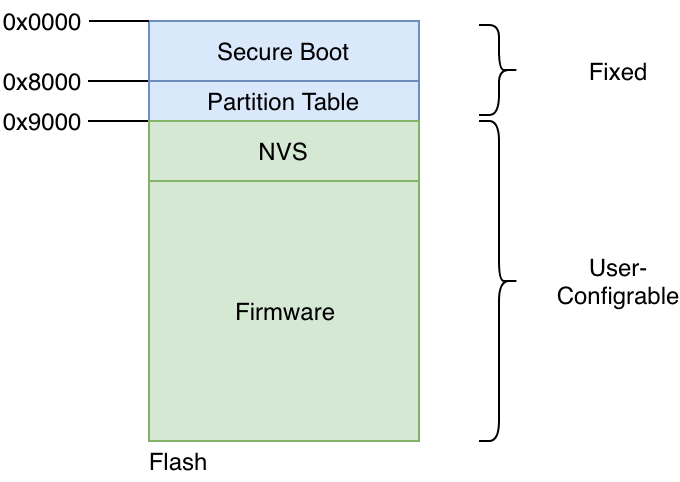
\includegraphics[scale=0.4]{Pictures/FlashPartitions_Intro.png}
    \caption{Flash Partitions Structure}
    \label{fig:flash_parts}
\end{figure}

As can be seen, the structure is static upto flash address 0x9000. The first part of the flash contains the second-stage bootloader, which is immediately followed by the partition table. The partition table then stores how the rest of the flash should be interpreted. Typically an installation will have at-least 1 NVS partition and 1 firmware partition.

\section{OTA Mechanism}\index{OTA Mechanism}
For firmware upgrades, an active-passive partition scheme is used. Two flash partitions are reserved for the 'firmware' component, as shown in the figure \ref{fig:ota_flash_parts}. The OTA Data partition remembers which of these is the active partition.

\begin{figure}[h!]
    \centering
    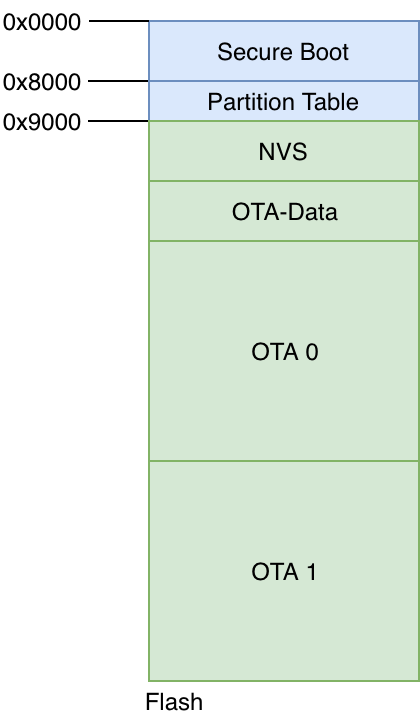
\includegraphics[scale=0.4]{Pictures/FlashPartitions_Upgrade.png}
    \caption{OTA Flash Partitions}
    \label{fig:ota_flash_parts}
\end{figure}

The typical state changes across the OTA firmware upgrade happens as shown in the figure \ref{fig:ota_workflow}. Behind the scene the following steps occur during the OTA upgrade workflow:
\begin{itemize}
    \item Step 0: OTA 0 is the active firmware. The OTA data partition stores this information as indicated.
    \item Step 1: The firmware upgrade process begins. The passive partition is identified, erased and new firmware is being written the OTA 1.
    \item Step 2: The firmware upgrade is completely written and verification is in-progress.
    \item Step 3: The firmware upgrade is successful, the OTA data partition is updated to indicate that OTA 1 is now the active partition. On the next boot-up the firmware from this partition will boot.
\end{itemize}

\begin{figure}[h!]
    \centering
    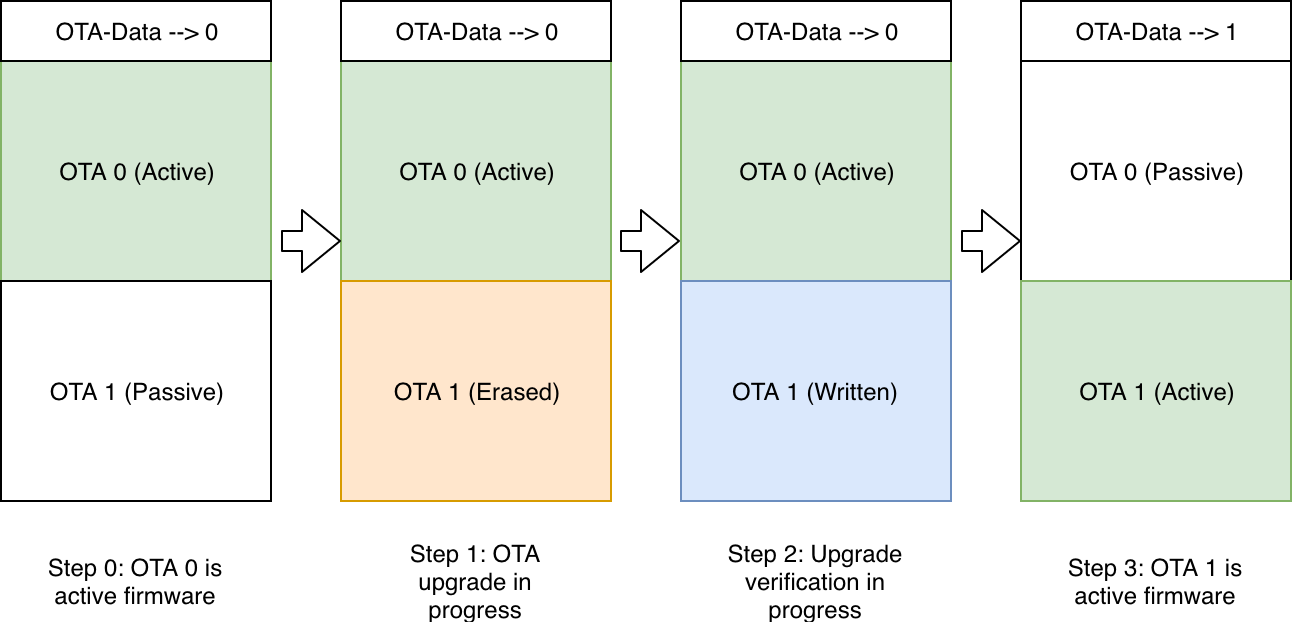
\includegraphics[scale=0.4]{Pictures/Upgrade_Flow.png}
    \caption{Firmware Upgrade Flow}
    \label{fig:ota_workflow}
\end{figure}

\subsection{Updating the Flash Partitions}\index{Updating the Flash Partitions}\label{sec:updating_flash_partitions}
So how exactly do we instruct the IDF to create a partition table that has this OTA-Data partition and the 2 partitions for storing the firmware?

This can be achieved by creating a partitions file. This is a simple CSV (Comma Separated Values) file that instructs IDF what are the partitions that we want, what should be their size and how should they be placed.

The partitions file that is used for this example is shown below:
\begin{minted}{text}

# Name,   Type, SubType, Offset,  Size, Flags
# Note: if you change the phy_init or app partition offset, make sure to change the offset in Kconfig.projbuild
nvs,      data, nvs,     ,        0x6000,
otadata,  data, ota,     ,        0x2000,
phy_init, data, phy,     ,        0x1000,
ota_0,    app,    ota_0,   ,      1600K,
ota_1,    app,    ota_1,   ,      1600K,
\end{minted}

The above partitions file instructs the IDF to create partitions: NVS, OTA-Data, OTA 0 and OTA 1, and it also specifies that sizes for each of these.

Once we create this partition file, we should instruct IDF to use this custom partitioning mechanism, over its default mechanism. This can be enabled by mentioned this detail in the SDK configuration. In the case of our application right now, this setting has already been activated in the \textit{6\_ota/sdkconfig.defaults} file. Hence you don't have to do any extra step for activating this.

But should you wish to use a different partitions file, or update the offset of the primary firmware, you should modify this setting. This can be done by executing the \textit{make menuconfig} command, and then configuring correct options in \textit{menuconfig} -> \textit{Partition Table}.

\section{The Code}\index{The Code}
Now let's check the code for enabling this functionality.

\begin{minted}{c}
    esp_http_client_config_t config = {
        .url = url,
        .cert_pem = (char *)upgrade_server_cert_pem_start,
    };
    esp_err_t ret = esp_https_ota(&config);
\end{minted}

\begin{itemize}
    \item The \textit{esp\_http\_client\_config\_t} structure is used to define the OTA upgrade source. This includes the URL that should be upgraded from, and also the CA certificate for validating the server from which the upgrade should be fetched. Please note that it is quite critical to ensure the validation of the CA certificate as mentioned in the Section \ref{sec:security_first}.
    \item The API \textit{esp\_https\_ota()} is then executed which initiates the firmware upgrade. When the firmware upgrade process is successful (or fails), this API returns with the appropriate error code.
\end{itemize}

The open question is how does the device receive the upgrade URL. The firmware upgrade command is typically different from the remote-control commands discussed in the earlier section. This is because the firmware upgrade is generally triggered by the device manufacturer for a batch or group of devices as they have identified.

You as the manufacturer can make the best choice about the appropriate manner for delivering the firmware upgrade notification to the device, and then calling the \textit{esp\_https\_ota()} API.

\section{Progress So Far}\index{Journey So Far}
With this firmware we enable a key feature of any smart connected device, the over-the-air firmware upgrade. 

Our product firmware is almost ready to be go, but for one any considerations for unique device data. Let's wrap that up in the upcoming Chapter.

\end{document}
